\subsection{Referenzszenario aktualisierte Kostensätze}

\subsubsection{Kenngrößen Szenario}

\captionof{table}{\label{table_4_kenngrößen_scenario} Basiskenngrößen Szenario 4}
\begin{center}
	\begin{tabularx}{\textwidth}{X | X } Kenngröße & Wert \\
	\hline
	Anzahl Untersuchungsgebiete & \num{154} \\
	Summe Streckenkilometer & \SI{13490.0}{\km}
	\end{tabularx}
\end{center}

\subsubsection{Kenngrößen Untersuchungsgebiete}
\captionof{table}{\label{table_4_kenngrößen_untersuchungsgebiete} Anzahl Untersuchungsgebiete sowie Kilometer nach Traktion 4}
\begin{center}
	\begin{tabularx}{\textwidth}{X | X | X} Traktion & Anzahl & Kilometer \\
	\hline
            electrification & \num{26} &  \SI{373.0}{\km}\\
            efuel & \num{0} &  \SI{0}{\km}\\
            battery & \num{102} &  \SI{6489.0}{\km}\\
            optimised electrification & \num{26} &  \SI{6629.0}{\km}\\
            diesel & \num{0} &  \SI{0}{\km}\\
            h2 & \num{0} &  \SI{0}{\km}\\
            no calculated cost & \num{0} &  \SI{0}{\km}\\
    	\end{tabularx}
\end{center}

\captionof{table}{\label{table_4_kenngrößen_untersuchungsgebiete_no_optimised} Anzahl Untersuchungsgebiete sowie Kilometer nach Traktion (Optimierte Elektrifizierung aufgeteilt) Szenario 4}
\begin{center}
	\begin{tabularx}{\textwidth}{X | X | X} Traktion & Anzahl & Kilometer \\
	\hline
            electrification & \num{26} &  \SI{3305.0}{\km}\\
            efuel & \num{0} &  \SI{0}{\km}\\
            battery & \num{102} &  \SI{10185.0}{\km}\\
            optimised electrification & \num{26} &  \SI{0}{\km}\\
            diesel & \num{0} &  \SI{0}{\km}\\
            h2 & \num{0} &  \SI{0}{\km}\\
            no calculated cost & \num{0} &  \SI{0}{\km}\\
    	\end{tabularx}
\end{center}
In dieser Tabelle wurden die Infrastrukturkilometer der Untersuchungsgebiete, bei denen die optimierte Elektrifizierung am wirtschaftlichsten war, auf die Traktionen Elektrifizierung und Batterie aufgeteilt (je nachdem, bei welchem Teiluntersuchungsgebiet welche Traktion am wirtschaftlichsten war)

\subsubsection{Kenngrößen Kosten}

\captionof{table}{\label{table_4_kenngrößen_untersuchungsgebiete_no_optimised} Investitionsvolumen sowie Betriebskosten (Barwert Preisstand 2016) Szenario 4}
\begin{center}
	\begin{tabularx}{\textwidth}{X | X | X} Traktion & Kosten Infrastruktur [Tsd. € Barwert] & Betriebskosten [Tsd. € Barwert]\\
	\hline
            electrification & \num{673314.0} &  \num{3515738.0}\\
            efuel & \num{0} &  \num{0}\\
            battery & \num{294200.0} &  \num{13887867.0}\\
            optimised electrification & \num{5834282.0} &  \num{23542479.0}\\
            diesel & \num{0} &  \num{0}\\
            h2 & \num{0} &  \num{0}\\
            no calculated cost & \num{0} &  \num{0}\\
    	\end{tabularx}
\end{center}

\begin{center}
	\begin{figure}[!h]
	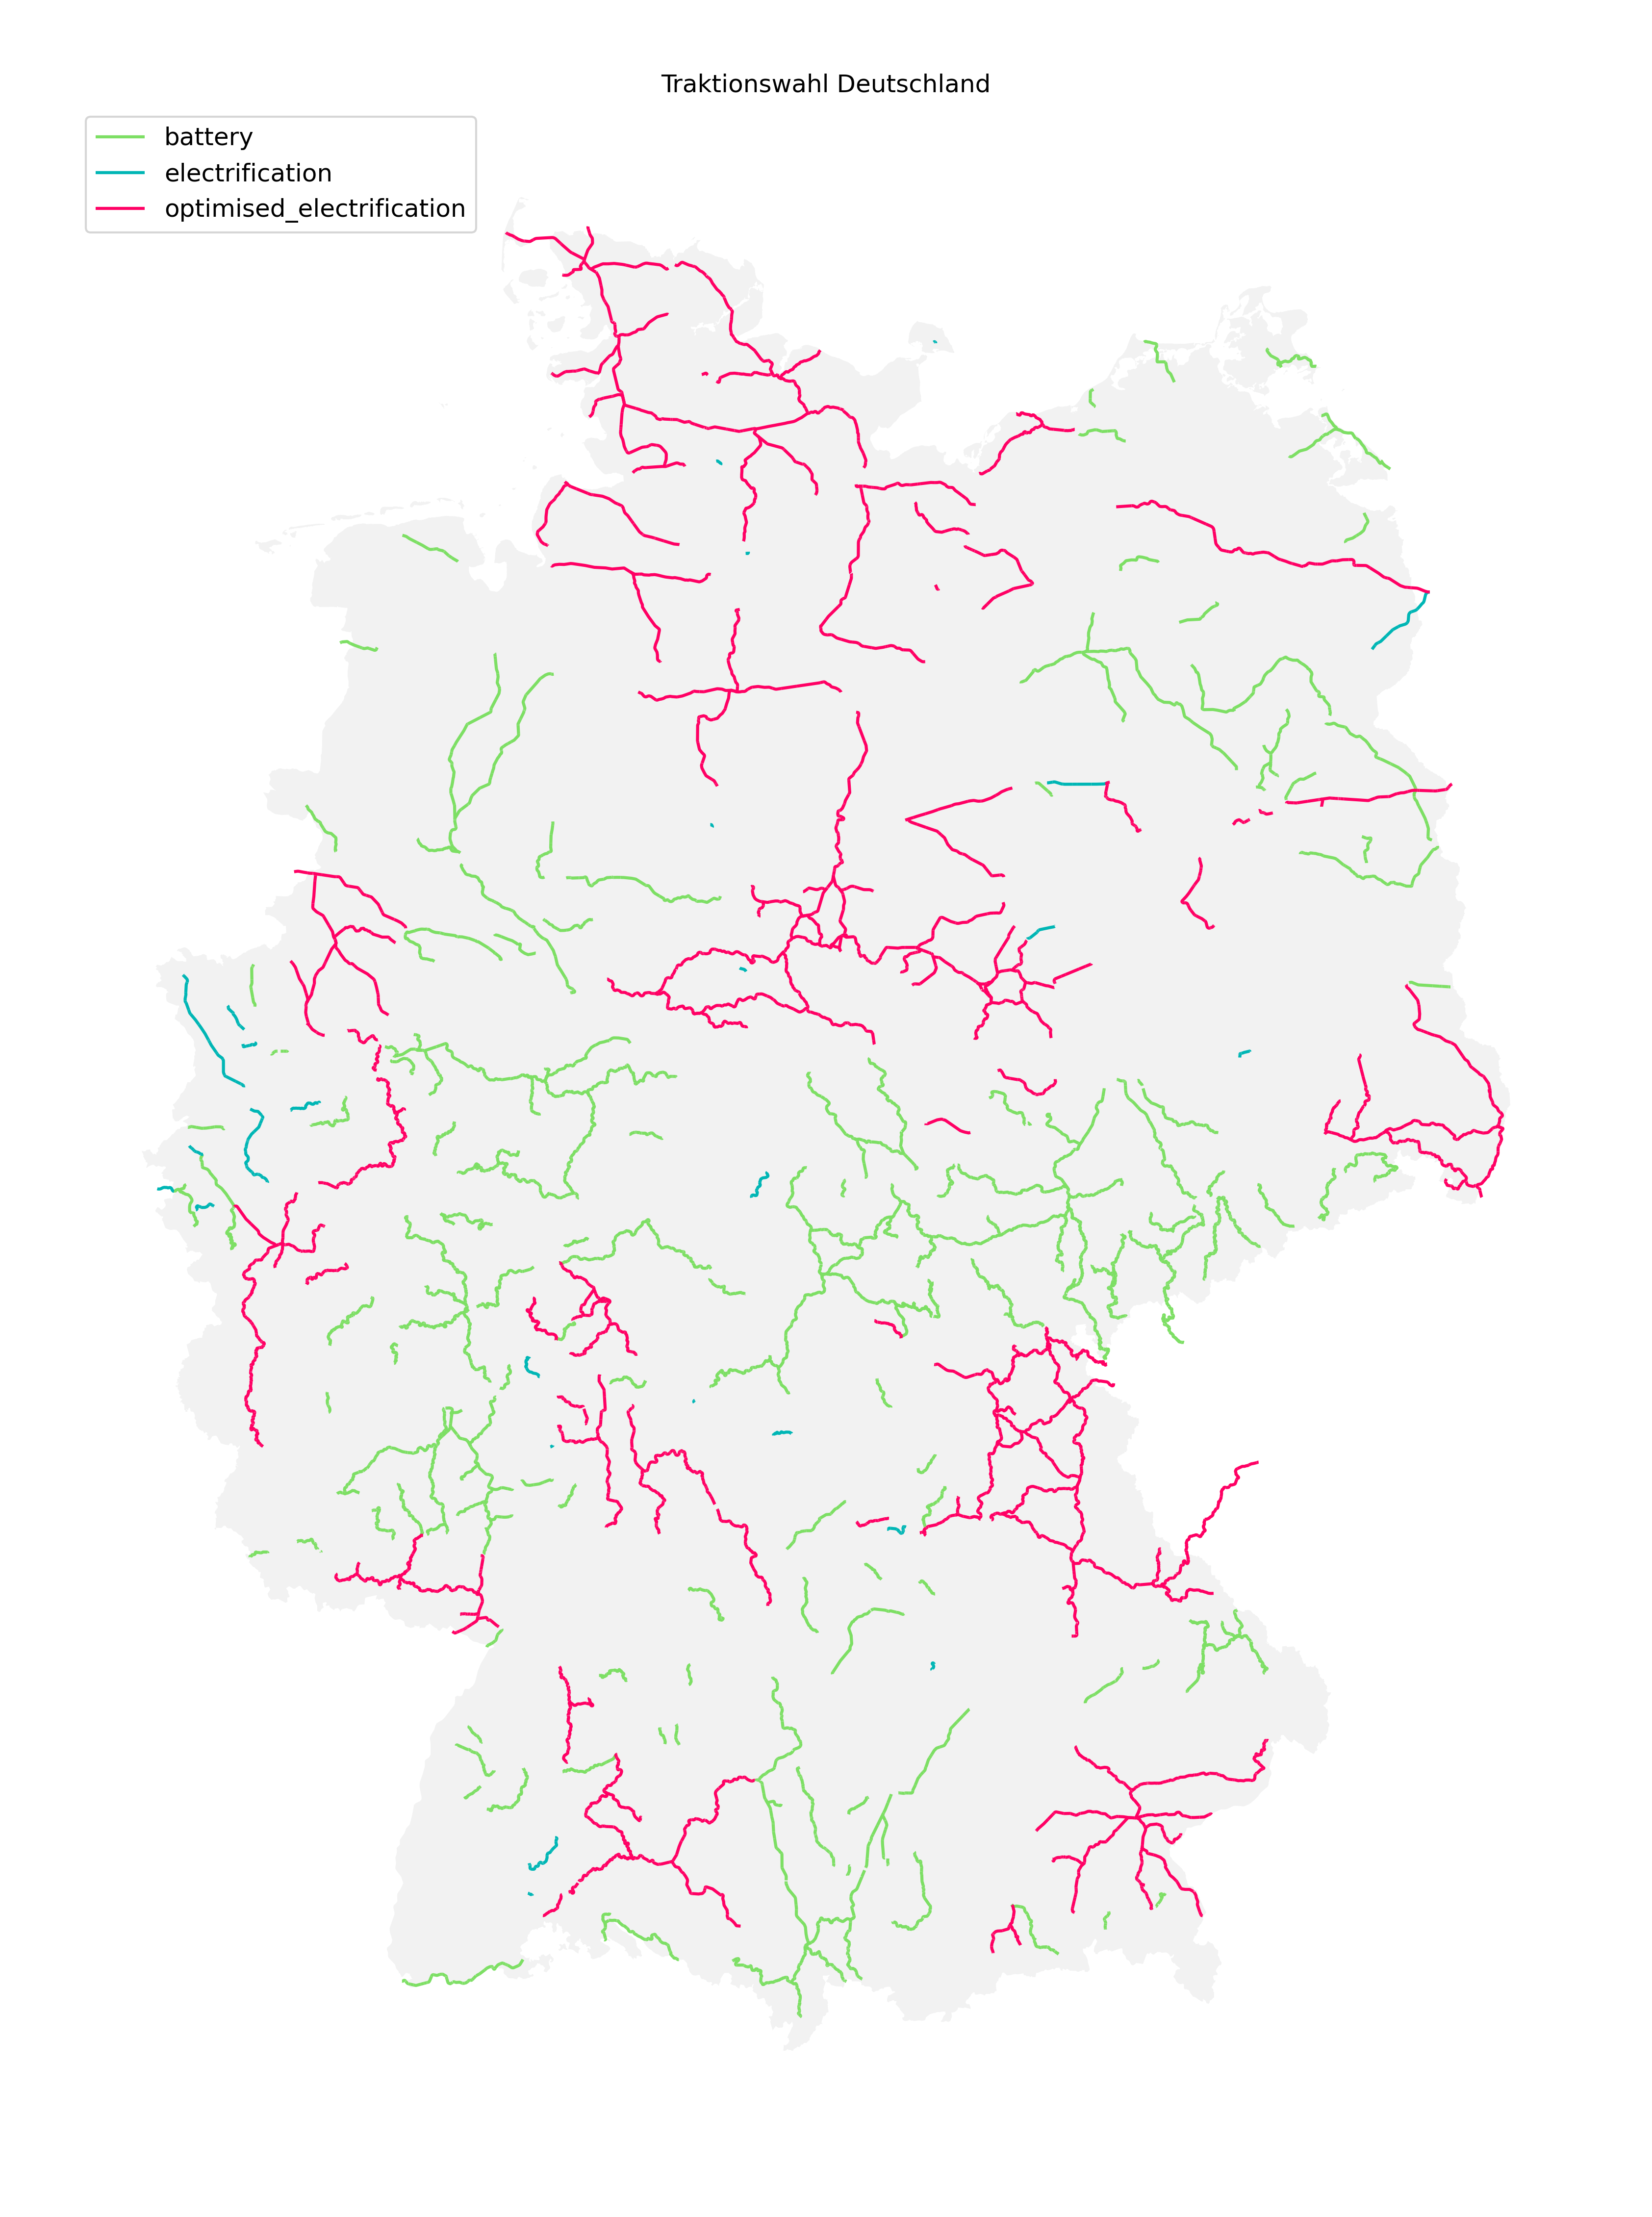
\includegraphics[height=0.8\paperheight]{../report_scenarios/s_4/files/deutschland_map.png}
	\caption{\label{fig_s_4_d_map} Karte Deutschland bevorzugte Traktion Untersuchungsgebiete Szenario 4}
	\end{figure}
\end{center}